\documentclass[10pt,a4paper]{article}
\usepackage[margin=20mm,headheight=13pt,headsep=10pt,footskip=14pt]{geometry}
\usepackage[T1]{fontenc}
\usepackage{lmodern}
\usepackage{amsmath,amssymb,mathtools,booktabs,graphicx,caption,microtype,fancyhdr,xcolor,hyperref}
\usepackage{enumitem}
\definecolor{navy}{HTML}{203550}
\definecolor{accent}{HTML}{177E89}
\hypersetup{colorlinks=true,urlcolor=accent,linkcolor=accent}
\pagestyle{fancy}
\fancyhf{}
\fancyhead[L]{\footnotesize\textcolor{navy}{HKUST\;|\;ISOM 3540}}
\fancyhead[R]{\footnotesize\textcolor{navy}{Assignment 4\;|\;Question 5}}
\fancyfoot[L]{\footnotesize Student ID: 21089310}
\fancyfoot[R]{\footnotesize Page \thepage}
\renewcommand{\headrulewidth}{0.35pt}
\renewcommand{\footrulewidth}{0pt}
\setlength{\parindent}{0pt}
\setlength{\parskip}{5.5pt}
\captionsetup{font=footnotesize,labelfont=bf}
\newcommand{\parthead}[1]{\vspace{2pt}\noindent\textcolor{navy}{\bfseries #1}\par\vspace{-2pt}}
\begin{document}
\begin{center}
 {\Large\bfseries ISOM 3540 -- Introduction to Probability Models}\\[4pt]
 {\large\bfseries Assignment 4: Solution to Question 5}\\[6pt]
 \begin{tabular}{@{}ll@{}}
 Student ID: & \textbf{21089310}\\
 Assignment deadline: & 16 November 2026\\
 \end{tabular}
\end{center}
\vspace{2pt}\hrule\vspace{10pt}

\textbf{Model and notation.} Let \(X\) be the number of interested customers and \(Y\) the number who purchase a policy. Under the assumptions in Question 5,
\[
 X\sim\operatorname{Bin}(100,0.5),\qquad
 Y\mid(X=x)\sim\operatorname{Bin}(x,0.3).
\]
Write \(A=\{12\leq Y\leq18\}\), and define \(g(x)=P(A\mid X=x)\).

\parthead{(a) Express the probability as an expectation of a function of \(X\).}
For each \(x\in\{0,\ldots,100\}\), the conditional binomial model gives
\[
 g(x)=
 \begin{cases}
 0, & 0\le x<12,\\[2pt]
 \displaystyle\sum_{y=12}^{\min\{18,x\}}
 {x\choose y}(0.3)^y(0.7)^{x-y}, & 12\le x\le100.
 \end{cases}
\]
By the law of total probability (or the tower property),
\begin{equation}
 \boxed{\;P(12\le Y\le18)=E[g(X)]
 =\sum_{x=0}^{100}{100\choose x}(0.5)^{100}g(x).\;}
 \label{eq:expectation}
\end{equation}
This is the requested expectation representation; it will also be the basis of the simulation.

\parthead{(b) Monte Carlo estimate using part (a).}
Use \(M=40{,}000\) independent replications and the fixed random seed \texttt{35402026}. The procedure is:
\begin{enumerate}[leftmargin=2em,itemsep=1pt,topsep=1pt]
\item Generate \(X_1,\ldots,X_M\) independently from \(\operatorname{Bin}(100,0.5)\).
\item For each realization \(X_i=x\), evaluate \(g(x)\) using the conditional binomial sum in (a).
\item Average the conditional probabilities rather than generating a second-stage \(Y_i\):
\end{enumerate}
\vspace{-8pt}
\[
 \widehat{p}_M=\frac{1}{M}\sum_{i=1}^{M}g(X_i)
 \quad\Longrightarrow\quad
 \boxed{\widehat{p}_{40{,}000}=0.67329525.}
\]
The sample standard error of this Monte Carlo mean is \(s_g/\sqrt{M}=0.00030768\), yielding the approximate 95\% simulation interval
\(\bigl[0.67269219,\,0.67389830\bigr]\). Because it averages conditional expectations, this estimator avoids the additional sampling variability from explicitly simulating \(Y\mid X\).

\begin{center}
 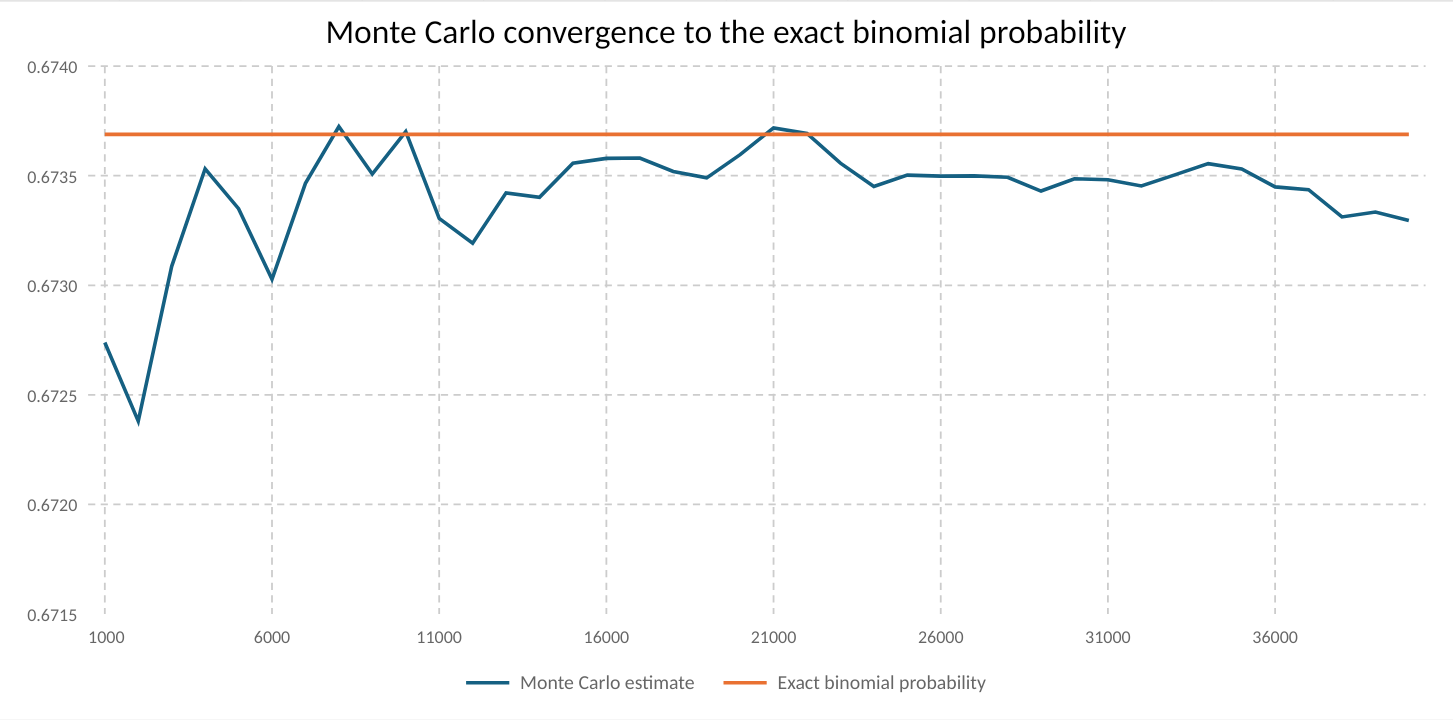
\includegraphics[width=0.86\linewidth]{ISOM3540_21089310_ass4_Excel_Convergence.png}\par
 \vspace{1pt}
 \captionof{figure}{Monte Carlo running estimate versus the exact binomial benchmark; chart created in Excel. The graph is a reproducibility aid, not an additional requirement of Question 5.}
\end{center}

\clearpage
\parthead{(c) Derive the marginal distribution of \(Y\) and find the exact probability.}
For \(y=0,\ldots,n\), the law of total probability gives
\begin{align*}
 P(Y=y)
 &=\sum_{x=y}^{n}P(Y=y\mid X=x)P(X=x)\\
 &=\sum_{x=y}^{n}{x\choose y}p_2^y(1-p_2)^{x-y}
                {n\choose x}p_1^x(1-p_1)^{n-x}.
\end{align*}
Using \({n\choose x}{x\choose y}={n\choose y}{n-y\choose x-y}\) and setting \(k=x-y\),
\begin{align*}
 P(Y=y)
 &={n\choose y}(p_1p_2)^y
   \sum_{k=0}^{n-y}{n-y\choose k}
   [p_1(1-p_2)]^k(1-p_1)^{n-y-k}\\
 &={n\choose y}(p_1p_2)^y
  [(1-p_1)+p_1(1-p_2)]^{n-y}\\
 &={n\choose y}(p_1p_2)^y(1-p_1p_2)^{n-y}.
\end{align*}
Therefore \(\boxed{Y\sim\operatorname{Bin}(n,p_1p_2)}\). Here \(n=100\) and \(p_1p_2=0.15\), so
\begin{equation}
 \boxed{\begin{aligned}
 P(12\le Y\le18)
 &=\sum_{y=12}^{18}{100\choose y}(0.15)^y(0.85)^{100-y}\\[-1pt]
 &=0.6736884056\;\approx\;0.67368841.
 \end{aligned}}
 \label{eq:exact}
\end{equation}
The Monte Carlo difference is \(\widehat p_{40{,}000}-P(A)=-0.00039316\), whose magnitude is about \(1.28\) estimated Monte Carlo standard errors. The two results are consistent.

\parthead{(d) Conditional probability that \(40\le X\le60\), given \(12\le Y\le18\).}
Let \(B=\{40\le X\le60\}\). By Bayes' rule and the definition of \(g(x)\),
\begin{align*}
 P(B\mid A)
 &=\frac{P(A\cap B)}{P(A)}
 =\frac{\displaystyle\sum_{x=40}^{60}P(X=x)P(A\mid X=x)}{P(A)}\\
 &=\frac{\displaystyle\sum_{x=40}^{60}{100\choose x}(0.5)^{100}
 \sum_{y=12}^{18}{x\choose y}(0.3)^y(0.7)^{x-y}}
 {\displaystyle\sum_{y=12}^{18}{100\choose y}(0.15)^y(0.85)^{100-y}}.
\end{align*}
Numerical evaluation yields \(P(A\cap B)=0.6574724968\) and \(P(A)=0.6736884056\). Thus
\begin{equation}
 \boxed{\;P(40\le X\le60\mid12\le Y\le18)
 =\frac{0.6574724968}{0.6736884056}
 =0.9759296603\;\approx\;\mathbf{0.97592966}.\;}
\end{equation}
\textbf{Independent check.} A customer is an interested non-buyer with probability \(0.5(0.7)=0.35\), a buyer with probability \(0.5(0.3)=0.15\), and otherwise uninterested. Conditional on \(Y=y\),
\[
 X\mid(Y=y)\;\overset{d}{=}\;y+\operatorname{Bin}\!\left(100-y,\frac{0.35}{0.85}\right).
\]
Summing this conditional distribution over \(y=12,\ldots,18\), weighted by \(P(Y=y\mid A)\), reproduces \(0.9759296603\), confirming the direct joint-probability calculation.

\vfill
\noindent\rule{\linewidth}{0.35pt}
{\footnotesize\textbf{Reproducibility and cited companion files.}\enspace
\href{https://github.com/YongWilliam-ai/ISOM3540_ass3_2026/blob/main/ISOM3540_ass4_2026/ISOM3540_21089310_ass4_MonteCarlo.xlsx}{Workbook}\enspace$\cdot$\enspace \href{https://github.com/YongWilliam-ai/ISOM3540_ass3_2026/blob/main/ISOM3540_ass4_2026/ISOM3540_21089310_ass4_Excel_Convergence.png}{Excel chart}\enspace$\cdot$\enspace \href{https://github.com/YongWilliam-ai/ISOM3540_ass3_2026/blob/main/ISOM3540_ass4_2026/ISOM3540_21089310_ass4.tex}{LaTeX source}\par\noindent \href{https://github.com/YongWilliam-ai/ISOM3540_ass3_2026/blob/main/ISOM3540_ass4_2026/reproduce_mc_ass4.py}{Reproducibility code}\enspace$\cdot$\enspace \href{https://github.com/YongWilliam-ai/ISOM3540_ass3_2026/blob/main/ISOM3540_ass4_2026/README.md}{README}\enspace$\cdot$\enspace \href{https://github.com/YongWilliam-ai/ISOM3540_ass3_2026/blob/main/ISOM3540_ass4_2026/ISOM3540_21089310_ass4_Complete_Package.zip}{Complete ZIP}.\par
\textit{The Excel workbook contains the 40,000 seeded simulation results, exact conditional-probability lookup, formulas and an editable convergence plot. The linked data and script enable verification of the reported results. All material for assessment is contained in this PDF.}}
\end{document}
